\documentclass[tikz,border=8pt]{standalone}
% Shared look for every TikZ diagram. Load with \input{../../tools/tikz-style.tex}
\usepackage[T1]{fontenc}
\usepackage{lmodern}
\renewcommand{\sfdefault}{lmr}  % diagrams use the same serif as the text
\usetikzlibrary{arrows.meta, positioning, shapes.geometric, calc, fit, backgrounds}
\definecolor{cblue}{HTML}{4C78A8}
\definecolor{corange}{HTML}{F58518}
\definecolor{cgreen}{HTML}{54A24B}
\definecolor{cred}{HTML}{E45756}
\definecolor{cpurple}{HTML}{B279A2}
\definecolor{cgrey}{HTML}{6B6B6B}
\tikzset{
  every picture/.style={font=\sffamily, line width=1.2pt},
  box/.style={draw=#1, fill=#1!12, rounded corners=4pt, align=center, inner sep=7pt, minimum height=1.1cm},
  box/.default=cgrey,
  arrow/.style={-{Stealth[length=3mm]}, draw=cgrey, line width=1.4pt},
  title/.style={font=\sffamily\bfseries\Large},
  note/.style={font=\sffamily\small, text=cgrey, align=center},
}
\AtBeginDocument{\hyphenpenalty=10000 \exhyphenpenalty=10000}

\begin{document}
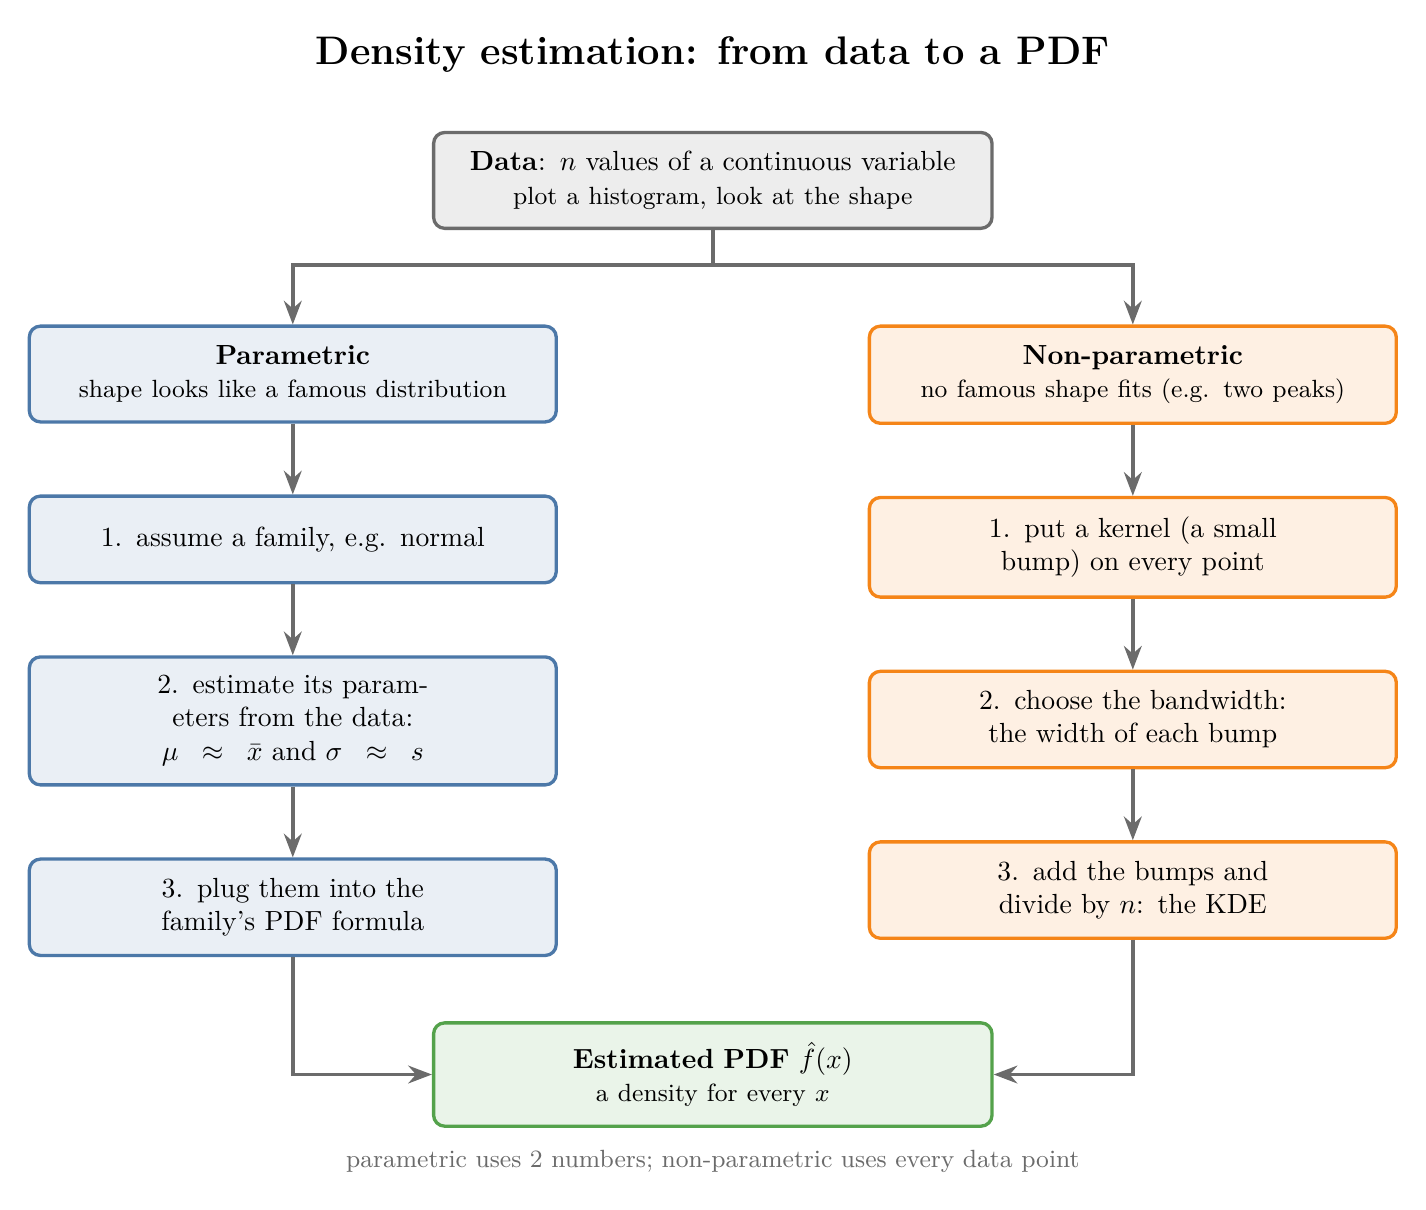
\begin{tikzpicture}[node distance=0.9cm and 0.8cm]
  \node[title] (t) {Density estimation: from data to a PDF};
  \node[box=cgrey, below=0.6cm of t, text width=6.6cm] (data) {\textbf{Data}: $n$ values of a continuous variable\\ \small plot a histogram, look at the shape};
  \node[box=cblue, below left=1.2cm and -1.6cm of data, text width=6.2cm] (p1) {\textbf{Parametric}\\ \small shape looks like a famous distribution};
  \node[box=corange, below right=1.2cm and -1.6cm of data, text width=6.2cm] (n1) {\textbf{Non-parametric}\\ \small no famous shape fits (e.g. two peaks)};
  \node[box=cblue, below=of p1, text width=6.2cm] (p2) {1. assume a family, e.g. normal};
  \node[box=cblue, below=of p2, text width=6.2cm] (p3) {2. estimate its parameters from the data:\\ $\mu \approx \bar{x}$ and $\sigma \approx s$};
  \node[box=cblue, below=of p3, text width=6.2cm] (p4) {3. plug them into the family's PDF formula};
  \node[box=corange, below=of n1, text width=6.2cm] (n2) {1. put a kernel (a small bump) on every point};
  \node[box=corange, below=of n2, text width=6.2cm] (n3) {2. choose the bandwidth: the width of each bump};
  \node[box=corange, below=of n3, text width=6.2cm] (n4) {3. add the bumps and divide by $n$: the KDE};
  \node[box=cgreen, text width=6.6cm] (pdf) at ($(p4.south)!0.5!(n4.south)+(0,-1.6)$) {\textbf{Estimated PDF} $\hat{f}(x)$\\ \small a density for every $x$};
  \draw[arrow] (data.south) -- ++(0,-0.45) -| (p1.north);
  \draw[arrow] (data.south) -- ++(0,-0.45) -| (n1.north);
  \foreach \a/\b in {p1/p2, p2/p3, p3/p4, n1/n2, n2/n3, n3/n4} \draw[arrow] (\a) -- (\b);
  \draw[arrow] (p4.south) |- (pdf.west);
  \draw[arrow] (n4.south) |- (pdf.east);
  \node[note, below=0.15cm of pdf] {parametric uses 2 numbers; non-parametric uses every data point};
\end{tikzpicture}
\end{document}
